\documentclass{standalone}

\usepackage[english]{babel}

% to define font size

\usepackage{ulem}
\usepackage{moresize}
\usepackage{anyfontsize}

% to use colors

\usepackage[dvipsnames]{xcolor}
\usepackage{MnSymbol}

\usepackage{listings}
\usepackage{lstvhdl}

% to use tikz and its libraries

\usepackage{tikz-timing}
\usepackage{tikz}

\usetikzlibrary{backgrounds}
\usetikzlibrary{positioning, calc, arrows, shapes, automata, petri, patterns,decorations.markings}
\usetikzlibrary{decorations.pathreplacing}

% to use tikzmark, to place and refer to marks outside the current figure

\tikzset{every picture/.style={remember picture}}

% styles for transitions

\tikzset{transition/.append style={fill=black!20, thick}}
\tikzset{transition/.append style={fill=black!20, thick}}

% styles for test and inhib arcs.

\tikzstyle{test}=[pre, *-]
\tikzstyle{inhib}=[pre, o-]

\usepackage{circuitikzgit}
\ctikzset{
  logic ports=ieee,
}

% Arrow positioning in a path

\tikzset{->-/.style={decoration={
  markings,
  mark=at position #1 with {\arrow{>}}},postaction={decorate}}}

\tikzset{-<-/.style={decoration={
  markings,
  mark=at position #1 with {\arrow{<}}},postaction={decorate}}}

% shift values

\newcommand{\outportshift}{0mm}
\newcommand{\outportidpshift}{0mm}

%%%%%%%%%%%%%%%%%%%%%%%%%%%%%%%%%%%%%%%%%%%%%%%%%%
%                  BEGIN DOCUMENT                %
%%%%%%%%%%%%%%%%%%%%%%%%%%%%%%%%%%%%%%%%%%%%%%%%%%

\begin{document}

\begin{circuitikz}

  \ctikzset{multipoles/dipchip/width=1.5}
  \ctikzset{multipoles/dipchip/pin spacing=.33}

  \node (pn) {
    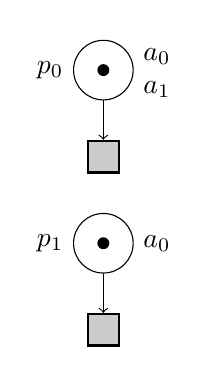
\begin{tikzpicture}

      % PLACES AND TRANSITIONS

      \node[place, tokens=1] (p0)  {};
      \node[transition, anchor=north] (t0) at ($(p0.south)-(0,.5)$) {};
      \node[place, tokens=1, anchor=north] (p1) at ($(t0.south)-(0,0.5)$) {};
      \node[transition, anchor=north] (t1) at ($(p1.south)-(0,.5)$) {};
      
      % LABELS

      \node[anchor=east] (pzLabel) at ($(p0.west)$) {$p_0$};
      \node[anchor=east] (poLabel) at ($(p1.west)$) {$p_1$};
      
      % ARCS
      \draw[->] ($(p0.south)$) -- ($(t0.north)$);
      \draw[->] ($(p1.south)$) -- ($(t1.north)$);

      % ACTIONS
      \node[anchor=west] at ($(p0.east)$) {
        \begin{tabular}{@{}l@{}}
          $a_0$ \\
          $a_1$ \\
        \end{tabular}
      };

      \node[anchor=west] at ($(p1.east)$) { $a_0$};      
    \end{tikzpicture}
  };

  % Output design
  \node (design) [draw, rectangle, inner sep=1mm] at ($(pn.east)+(5.5,0)$) {
    \begin{tikzpicture}
      
      % Actions process

      \node[draw, rectangle, inner sep=10pt] (actionsps)  {
        \begin{lstlisting}[language=VHDL, frame=]
rst {
  $\gamma(a_0)$ <= false;
  $\gamma(a_1)$ <= false
} else {
  falling {
    $\gamma(a_0)$ <= or($id_{m_0}$, $id_{m_1}$);
    $\gamma(a_1)$ <= $id_{m_0}$
  }
}
\end{lstlisting}
      };

      \node[anchor=south west] at ($(actionsps.north west)$) {$\mathtt{actions}$};
      
      % PDI idp0
      
      \draw       
      node [dipchip, num pins=4, hide numbers,
      no topmark, external pins width=0, anchor=south east]
      (idp0) at ($(actionsps.north west)-(1,1)$) {
        
      };

      \node[anchor=south] at ($(idp0.north)$) {$\gamma(p_0)$};

      \draw ($(idp0.east)$)
      node [anchor=east, font=\ssmall, inner sep=1mm]  {\tt marked};

      % PDI idp1
      
      \draw       
      node [dipchip, num pins=4, hide numbers,
      no topmark, external pins width=0, anchor=north east]
      (idp1) at ($(actionsps.south west)-(1,-1)$) {
        
      };

      \node[anchor=south] at ($(idp1.north)$) {$\gamma(p_1)$};

      \draw ($(idp1.east)$)
      node [anchor=east, font=\ssmall, inner sep=1mm]  {\tt marked};

      % INTERCONNECTIONS

      \draw[red,->-=.5] ($(idp0.east)$) --++(.3,0)  |- ($(actionsps.west)+(0,.3)$) node[midway, yshift=-5pt, font=\ssmall] {$id_{m_0}$};
      \draw[red,->-=.5] ($(idp1.east)$) --++(.3,0)  |- ($(actionsps.west)-(0,.3)$) node[midway, xshift=-8pt, font=\ssmall] {$id_{m_1}$};
      % \draw[red,->-=.5] ($(idp0.bpin 3)$) --++(.3,0) |- ($(idt1.bpin 1)$);
      % \draw[red,-<-=.5] ($(idp0.bpin 1)$) -|++ (-.3, 1.7) -| ($(idt0.east)+(.3,0)$) -- (idt0.east);
      % \draw[red,-<-=.5] ($(idp0.bpin 2)$) -|++ (-.3, -1.2) -| ($(idt1.east)+(.3,0)$) -- (idt1.east);
      
    \end{tikzpicture}
    \hspace*{20pt}    
  }; 

  % ACTION OUTPUT PORTS
  
  \draw[red, ->-=.5] ($(actionsps.12)$) --++ (1.2, 0) node[anchor=west,above, xshift=5pt] { $\gamma(a_0)$ };
  \draw[red, ->-=.5] ($(actionsps.-12)$) --++ (1.2, 0) node[anchor=west,above, xshift=5pt] { $\gamma(a_1)$ };
  
  % TRANSLATION ARROW
  
  \node at ($(pn.east)!.3!(design.west)$) {\Huge$\rightarrow$};
  
\end{circuitikz}

\end{document}

%%% Local Variables:
%%% mode: latex
%%% TeX-master: t
%%% End:
